\section{Atoms and Molecules}
	The attention concerning atoms has been on three single atoms, helium, beryllium and neon, and two molecules, dihelium ($\mbox{He}_2$) and diberyllium ($\mbox{Be}_2$). In this section different optimizations of the VMC solver will be tested, and ground state energies and one-body densities will be calculated. There will also be a comparison to calculations using gaussian type orbitals, and a statistical discussion, using blocking.
	
	%\todo{short intro}

	\subsection{Optimization results}
		By using an analytical expression for the local energy instead of using a numerical derivation in the calculation the program becomes more efficient. For Helium we achieve a speedup of nearly 48 percent, while for Beryllium a speedup of approximately 80 percent is achieved, see Table \ref{tab:analyticVSNumeric}.

		\begin{table}
			\center
			\begin{tabular}{ c | c | c | c }
			    %\hline
			   	\textbf{Trialfunction} & Numerical (s) & Analytical (s) & Ratio
			    \\ \hline
			    Helium $\psi_{T}$ & 29.7288 & 20.1189	& 0.6767\tabularnewline
			    %\\	\hline
			    Beryllium $\psi_{T2}$ & 58.9623  &	32.4622 & 0.5505\tabularnewline
				%\\ \hline
			\end{tabular}
			\caption{The time to run a Monte Carlo run with \(10^7\) cycles for Helium, and \(10^6\) cycles for Beryllium. Using an analytical expression for the local energy decreases the computation time by a significant degree for both trialfunctions tested. }
			\label{tab:analyticVSNumeric}
		\end{table}

	\subsection{Speedup with MPI}
		\begin{table}
			\center
			\begin{tabular}{ c | c| c| c| c}
				%\hline
				\textbf{Num. of processes} &	1	&	2	&	3	&	4
				\\ \hline
				Speedup	&	1.0	&	1.97	&	2.90	&	3.35
				%\hline
			\end{tabular}
			\caption{Speedup achieved by using MPI to run computations on multiple processors.}
			\label{tab:MPI_speedup}
		\end{table}

		\begin{figure}
			\centering 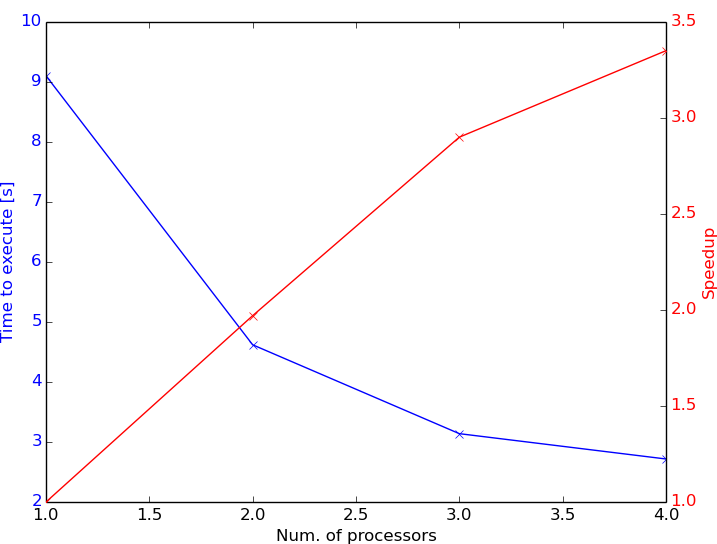
\includegraphics[width=0.49\linewidth]{content/Results/figures/processor_number_time_comparison}
			\protect\caption{Using MPI, the time used as a function of number of processors used, and the corresponding speedup achieved.}
			\label{fig:MPI_speedup}
		\end{figure}

		It is desirable to have a speedup as close as possible
                to the number of processors used. The speedup measured
                by our VMC program running 1, 2, 3 and 4 processors is shown in
                Table \ref{tab:MPI_speedup} and
                Fig. \ref{fig:MPI_speedup}. We see that the speedup is
                good for 2 and 3 processes, in that it is almost equal
                to the number of processes used. However when running
                4 processes the speedup gain suffers somewhat. This is
                because the computer has only 4 processors, so running
                on all processors the VMC program has to share
                resources with the operating system and other
                programs. However, this simple implementation of our parallel version of the code on standard quad-core PC which can be bought in any supermarket, demonstrates the ease by which Monte Carlo methods can be run in parallel. 

	\subsection{Using brute force Monte Carlo sampling}
		As a first attempt to solve the ground state energy for the helium
		atom we perform Variational Monte Carlo calculation with a brute force
		Metropolis sampling. We do this with two trial wave functions
		\[
		\psi_{T}({\bf r_{1}},{\bf r_{2}},{\bf r_{12}})=\exp{\left(-\alpha(r_{1}+r_{2})\right)}\exp{\left(\frac{r_{12}}{2(1+\beta r_{12})}\right)},
		\]
		using $\alpha$ and $\beta$ as variational parameters. 
		We run the Variational Monte Carlo calculation over
		different values for the two variables $\alpha$ and $\beta$, 
		with $2\times10^{7}$ cycles in the Monte Carlo simulation, and the resulting energies are
		presented in Fig. \ref{fig:HeliumAlphaBeta}.
		
		We find the optimal values to be  $\alpha=1.843$ and $\beta=0.34$, as we can see in the figures.
		Using these values for $\alpha$ and $\beta$ we run the brute force variational Monte Carlo calculation. The program finds an optimal value for the steplength, $\delta$, which results in roughly 50 percent accepted moves. Using $10^{8}$ cycles the algorithm finds the steplength to be $\delta = 1.5$, giving 48.8 percent accepted moves. The energy found with this method is $-2.89024$, with a variance of $3.77402\times10^{-5}$, as presented in Table \ref{tab:Helium_no_IS}.
		The parameter $\alpha$ can be interpreted as a parameter for the
		force pulling the electron to the nucleus.

		\begin{table}
			\center
			%\resizebox{\linewidth}{!}{%
			\begin{tabular}{c|c|c|c}
			    %\hline
			   	Atom  & $\mbox{E}_{\mbox{\scriptsize{VMC}}}$ & Variance & $\mbox{E}_{\mbox{\scriptsize{ref}}}$ \tabularnewline
				\hline 
				Helium & $-2.89024$ & $3.77402\times10^{-5}$ & $-2.9037$ \tabularnewline
				%\hline 
			\end{tabular}%}
			\caption{Ground state energy for Helium calculated with variational Monte Carlo without using Importance Sampling. The reference energy is from Ref. \cite{Binkley_1975}.}
			\label{tab:Helium_no_IS}
		\end{table}
		


		\begin{figure}
			\centering 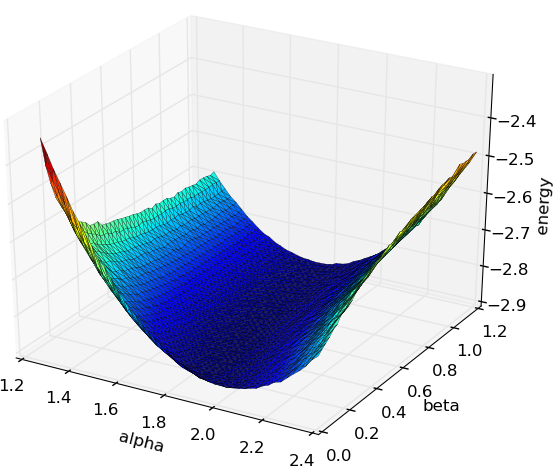
\includegraphics[width=0.49\linewidth]{content/Results/figures/HeliumJastrowAnalytical_alpha_beta_energy}
			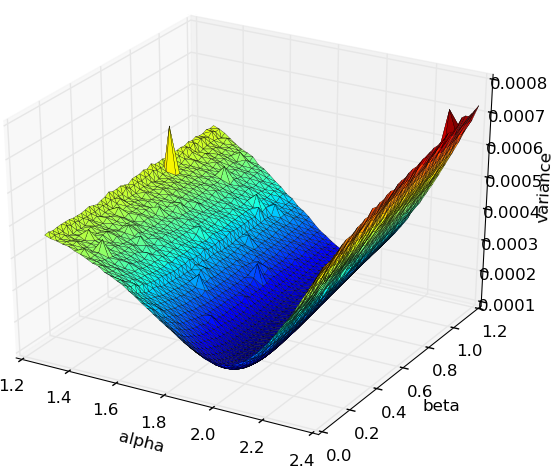
\includegraphics[width=0.49\linewidth]{content/Results/figures/HeliumJastrowAnalytical_alpha_beta_variance}
			\protect\caption{For helium using $\psi_{T}$, the energy as a function of alpha and beta (left), and the variance as a function of $\alpha$ and $\beta$. }
			\label{fig:HeliumAlphaBeta}
		\end{figure}

	\subsection{Ground state energies}
		We now introduce importance sampling to our calculations of the Helium atom, and expand the calculations to the Beryllium and the Neon atoms, and the Helium and the Beryllium molecules. 

		%From a search for the optimal variables for Helium, we find them to be $\alpha=1.843$ and $\beta=0.34$. , we get an energy of $-2.89012$ and a corresponding variance $7.76888\times10^{-5}$, 
		Expanding the system to larger atoms, we use the trial functions given in Eq. \eqref{eq:BerylliumTrialFunction} for Beryllium, and Eq. \eqref{eq:NeonTrialFunction} for Neon. Optimal values for $\alpha$ and $\beta$ are found by variation until the ground energy is minimized. The resulting ground state energies of the systems are presented in Table \ref{tab:EnergyAlphaBetaReference}. There is a relatively large uncertainty of the ground state energies, especially for Neon and the molecules, because the variance of the energy compared to the difference in energy caused by varying the parameters is quite high. However, as a function of the variational parameters the variance is more smooth, see fig \ref{fig:HeliumAlphaBeta}, and it is therefore easier to determine the best values for the variables from variance as a function of \(\alpha\) and \(\beta\). The energy and variance as a function of the timestep, $\delta t$ is shown in Fig. \ref{fig:HeliumTimestep}. 

		The ground state energies found with the variational Monte Carlo method are in good agreement with the reference energies. However the method generally underestimates the ground state energies. There is also a big statistical error, increasing with the size of the systems, which stems from a relatively low number of Monte Carlo samples. 


		\begin{figure}
			\centering 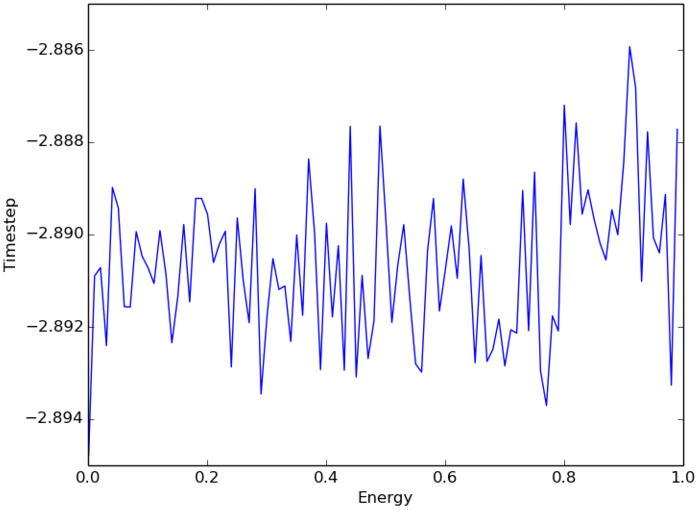
\includegraphics[width=0.49\linewidth]{content/Results/figures/HeliumJastrowAnalyticalTimeEnergy}
			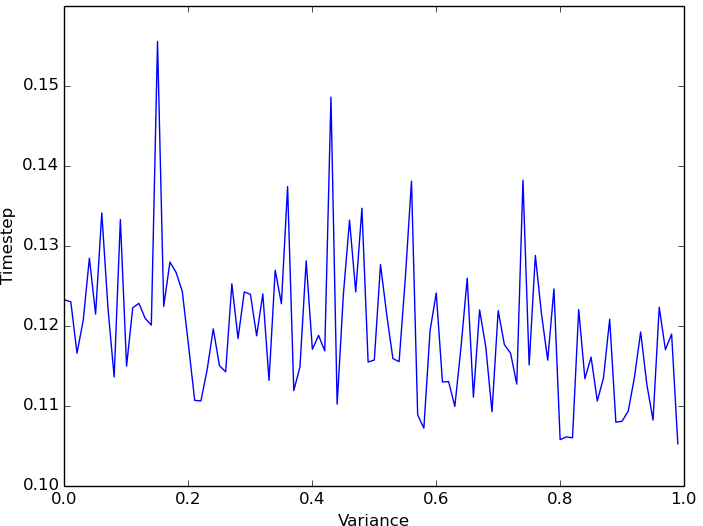
\includegraphics[width=0.49\linewidth]{content/Results/figures/HeliumJastrowAnalyticalTimeVariance}
			\protect\caption{For helium $\psi_{T}$, timestep shown as a function of energy (left) and variance (right), using $\alpha = 1.84$ and $\beta=0.34$.}
			\label{fig:HeliumTimestep}
		\end{figure}

		\begin{figure}
			\centering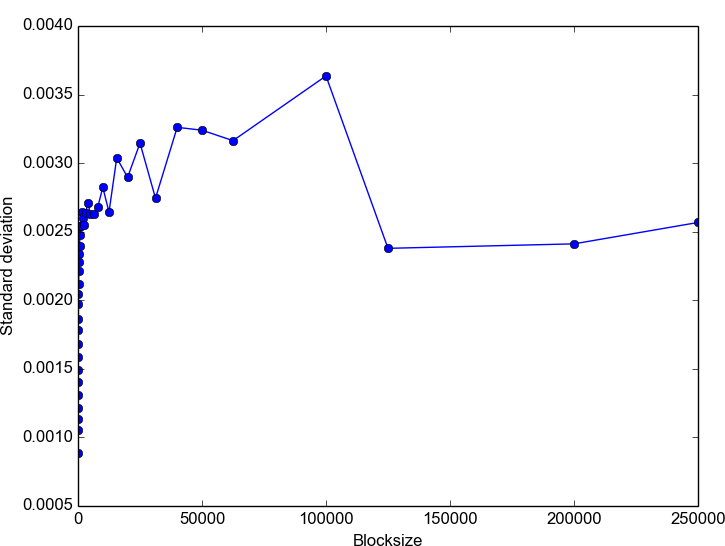
\includegraphics[width=0.49\linewidth]{content/Results/figures/Helium_blocking}
			\protect\caption{Statistical analysis for the helium case, using blocking. The blocking behaviour can be seen very clearly as it plateaus rapidly with increasing blocksize.}
			\label{fig:HeliumBlocking}
		\end{figure}


		\begin{figure}
			\centering 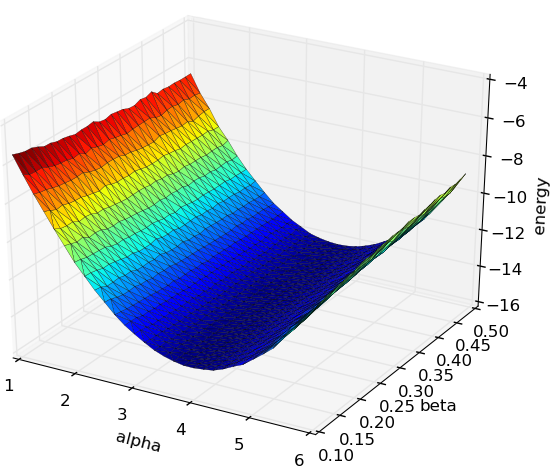
\includegraphics[width=0.49\linewidth]{content/Results/figures/Beryllium_alpha_beta_energy}
			\centering 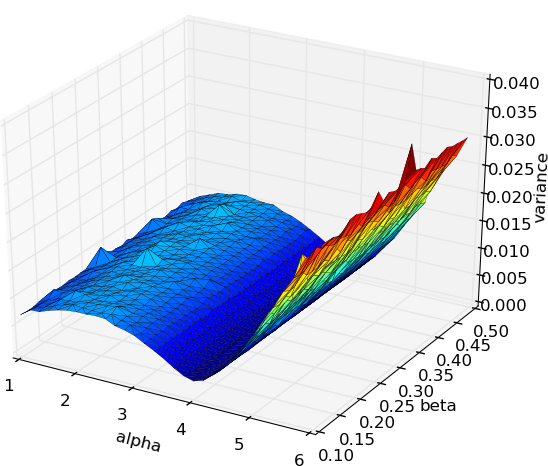
\includegraphics[width=0.49\linewidth]{content/Results/figures/Beryllium_alpha_beta_variance}
			\protect\caption{Energy (left) and variance (right) as a function of $\alpha$ and $\beta$ for Beryllium, using $10^{6}$ cycles.}
			\label{fig:alpha_beta_comparison_beryllium}
		\end{figure}

		\begin{figure}
			\centering 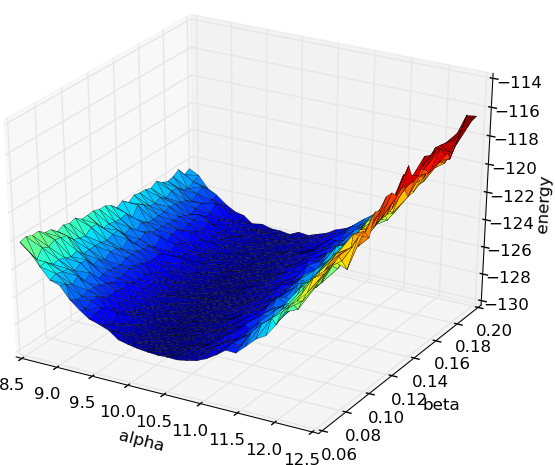
\includegraphics[width=0.49\linewidth]{content/Results/figures/Neon_alpha_beta_energy}
			\centering 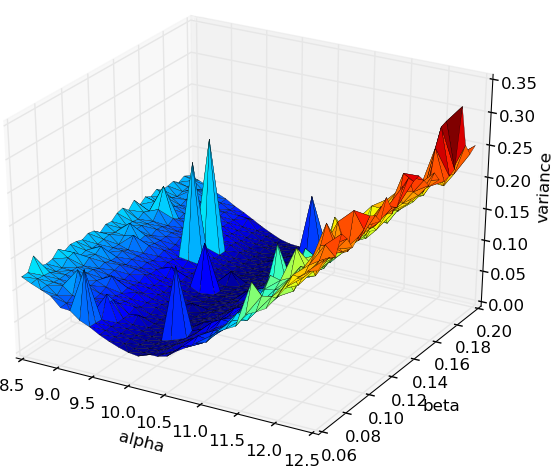
\includegraphics[width=0.49\linewidth]{content/Results/figures/Neon_alpha_beta_variance}
			\protect\caption{Energy (left) and variance (right) as a function of $\alpha$ and $\beta$ for Neon, using $10^{5}$ cycles.}
			\label{fig:alpha_beta_comparison_neon}
		\end{figure}

		To find optimal $\alpha$ and $\beta$ values for the atoms we
                run VMC with ranges of different values for \(\alpha\)
                and \(\beta\). The resulting plots of the variance and  the
                energy for different combinations are given in
                Fig. \ref{fig:alpha_beta_comparison_beryllium} for
                Beryllium and
                Fig. \ref{fig:alpha_beta_comparison_neon} for Neon. As
                VMC runs slowly for Neon, because it has ten electrons,
                we made runs over the range of Alpha and
                Beta values with $10^{5}$ cycles. This is reflected in
                the higher variance, and the spikes in the variance
                plot.

		\begin{table}
			\center %
			%\resizebox{\linewidth}{!}{%
			\begin{tabular}{c|c|c|c|c}
				%\hline 
				Atom  & $\mbox{E}_{\mbox{\scriptsize{VMC}}}$ & Variance & $\mbox{E}_{\mbox{\scriptsize{ref}}}^{(a)}$ & $\mbox{E}_{\mbox{\scriptsize{ref}}}^{(b)}$ \tabularnewline
				\hline 
				He & $-2.89012$ & $7.77\times10^{-5}$ & $-2.9037$ & $-2.9036(2)$\tabularnewline
				%\hline 
				Be & $-14.3902$  & $9.09\times10^{-4}$ & $-14.667$ & $-14.657(2)$ \tabularnewline
				%\hline 
				Ne  & $-127.875$ & $0.0132$ & $-128.928$ & $-128.765(4)$ \tabularnewline
				%\hline 
				H$_2$ &   $-1.15828$	& $0.00023$  & $-1.17540$ & $-1.1745(3)$ \tabularnewline
				%\hline
				Be$_{2}$   & $ -31.349 $	& $ 0.0076 $  & $-29.339$ & $-29.301(5)$ \tabularnewline
				%\hline
			\end{tabular}%}
			\protect\caption{Ground state energies of atoms and molecules, computed with the variational Monte Carlo method. For H$_2$ and Be$_2$ we used a nuclei distance of \( 1.40 \) and \( 4.63\), respectively.  Refs. (a): \cite{Koput_2011_PCCP} \cite{Binkley_1975}, (b): \cite{hogbergetDMC} (using diffusion Monte Carlo).}
			\label{tab:EnergyAlphaBetaReference} 
			%The binding enery found for Be\(_2\) is too low which is caused by a bug in the implementation of the molecule.
		\end{table}

		\begin{figure}
			\centering 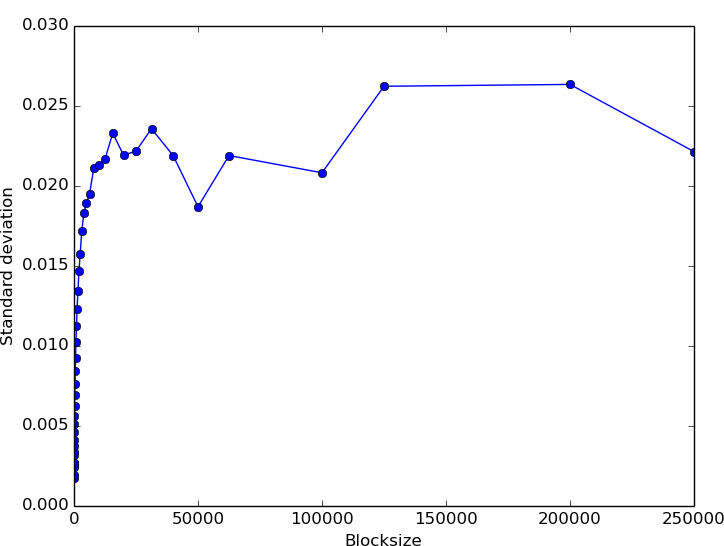
\includegraphics[width=0.49\linewidth]{content/Results/figures/Beryllium_blocking}
			\centering 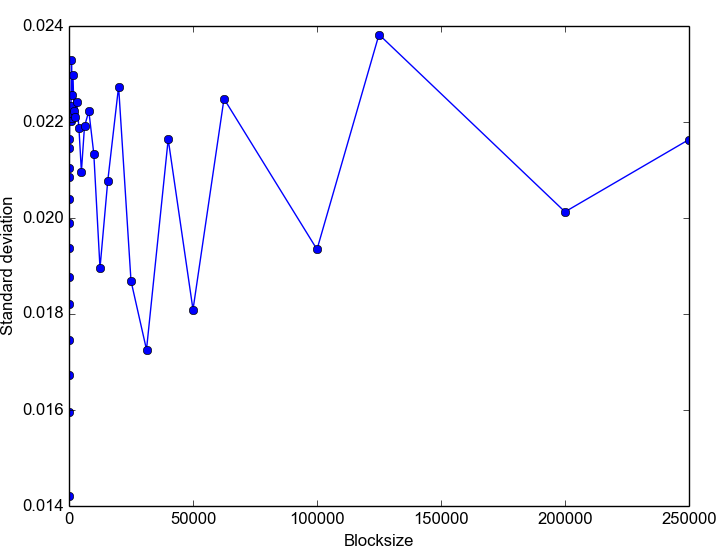
\includegraphics[width=0.49\linewidth]{content/Results/figures/Neon_blocking}
			\protect\caption{Statistical analysis of beryllium using blocking with $10^6$ Monte Carlo cycles. There is a clear plateauing behaviour as the blocksize increases after rising dramatically for small blocksizes. This is due to the blocksize catching up to the correlation length between the measurements. \todo{NB!!}}\label{fig01:std_Stuff}
		\end{figure}



	\subsection{Using Gaussian Type Orbitals}
		Using GTOs we can nearly reproduce the energies we get
                from using Slater Type Orbitals, although with GTOs
                not quite as low energies are reached. This is due to
                the GTOs being an imperfect representation of the
                STOs. Using GTOs in stead of STOs is also considerably
                slower, as seen in \ref{tab:AtomsGTO}. This can be due
                to inefficient code, and there is also room for
                improvements by calculating analytical derivatives of
                the GTOs. However using GTOs reduces the variables to
                only $\beta$, thus we don't have to look for energy
                minima by varying $\alpha$. This means that it is
                possible to easily use a gradient method to more
                efficiently find the variable that gives minimum
                energy.

		\begin{table}
			\center %
			\resizebox{\linewidth}{!}{%
			\begin{tabular}{c|c|c|c|c|c|c}
				%\hline 
				Atom &  $\mbox{E}_{\mbox{\scriptsize{VMC}}}$ & Var. & $\mbox{E}_{\mbox{\scriptsize{ref}}}^{(a)}$ & $\mbox{E}_{\mbox{\scriptsize{ref}}}^{(b)}$ & GTO [s] & STO [s] \tabularnewline
				\hline 
				He &  $-2.85482$ & $0.004$ & $-2.9037$ & $-2.9036(2)$ & $15.0$ & $6.5$ \tabularnewline
				%\hline 
				Be  & $-14.0182$ & $0.002$ & $-14.667$ & $-14.657(2)$ & $48321$ & $4141$ \tabularnewline
				%\hline 
				Ne  & $-113.542$ & $0.498$ & $-128.928$ & $-128.765(4)$ & $2821$ & $203$ \tabularnewline
				%\hline 
			\end{tabular}}
			\protect\caption{ Comparison of energies found using bisection method with the refenrence energy \cite{Koput_2011_PCCP} \cite{Binkley_1975} and comparison of the time used running the computation with the given number of cycles using GTOs and STOs.}
			\label{tab:AtomsGTO} 
		\end{table}

	\subsection{One-body densities}
		\subsubsection{Helium Atom}
			Simulations of the helium atom have been
                        studied using several different
                        trialfunctions. First the electrons are
                        regarded as having pure hydrogenlike
                        wavefunctions. Then the hydrogenlike
                        wavefunctions are expanded by optimizing the
                        \(\alpha \) value to get a better ground state
                        energy. For the final calculations the
                        Padé-Jastrow correlation factor is added to
                        include the effects of the electron-electron
                        repulsion. The results of the case without
                        Padé-Jastrow correlation is presented in Table
                        \ref{tab:helium_wavefunctions_tests}. Note
                        that the variance listed is the variance for
                        the local energy between each particle moves in
                        the VMC calculations, not the true variance, which is
                        obtained through the blocking routine
                        described in section \ref{sec:blocking}.

			In Fig. \ref{fig:HeliumoneBodyDensity}
                        histograms of the positions the electrons
                        occupy during the simulations are presented,
                        and we can see that for the pure hydrogenic
                        wavefunction the electrons are generally
                        closer to the nucleus than in the other two
                        simulations. The ground-state energy improved
                        and got closer to the reference value, as
                        listed in \ref{tab:EnergyAlphaBetaReference},
                        as the wavefunction got more sophisticated,
                        and we have a decreasing variance. In the
                        wavefunction the $\alpha$ parameter represents
                        the electrical attraction of the nucleus on
                        the electron, and represents an effective charge.
In a real Helium atom the
                        attraction felt by the electrons is smaller
                        than the charge of the nucleus because it is
                        also under the influence of the other
                        electrons. For the Helium atom the effect of
                        the correlation factor is not very pronounced,
                        because there are only two electrons, and they
                        can be quite far away from each other. However
                        the correlation factor is still significant in
                        the ground-state energy and the variance.

			\begin{table}
			\center %
			%\resizebox{\linewidth}{!}{%
			\begin{tabular}{c|cc}
				%\hline 
				Atom & $\mbox{E}_{\mbox{\scriptsize{VMC}}}$ &Var. \tabularnewline
				\hline 
				He &  $-2.757$ & $0.0030$ \tabularnewline
				Be &  $-13.710$ & $0.0072$ \tabularnewline
				Ne &  $-110.301$ & $0.0477$ \tabularnewline

			\end{tabular}%}
			\protect\caption{ Energies for the helium, beryllium and neon atoms using simple helium wavefunctions with only one variational parameter. Note that the variance is the variance for the local energy between each particle move, not the true variance.}
			\label{tab:helium_wavefunctions_tests} 
			\end{table}

			\begin{figure}
					\centering 
					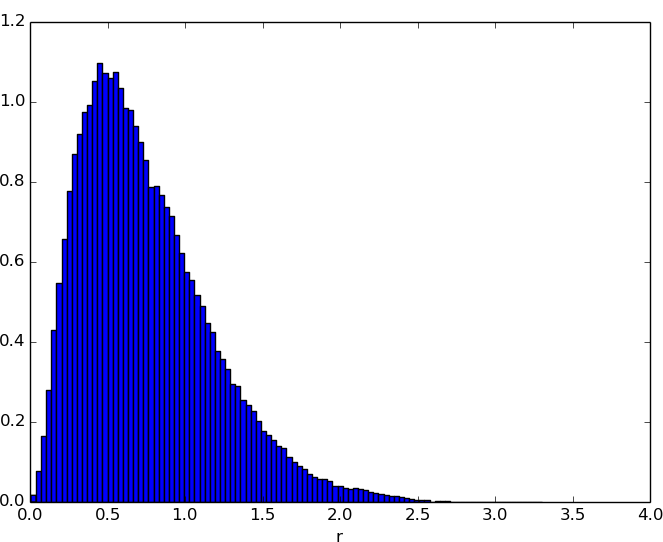
\includegraphics[width=0.32\linewidth]{content/Results/figures/ChargeDensityHeliumHydrogenic}
					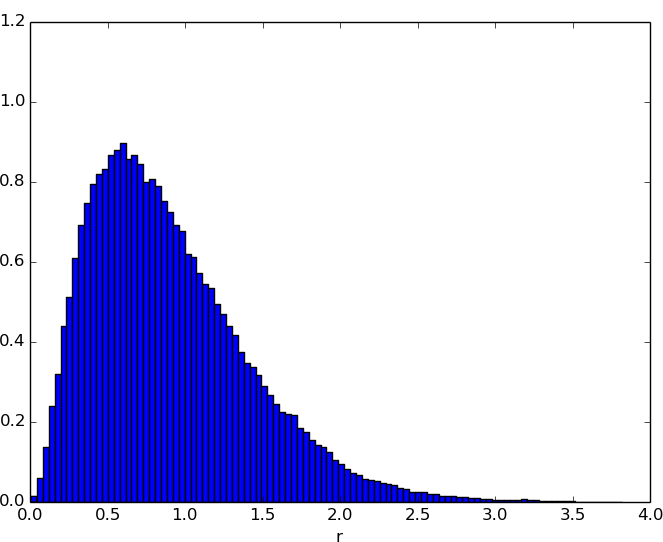
\includegraphics[width=0.32\linewidth]{content/Results/figures/ChargeDensityHeliumSimpleAnalytical}
					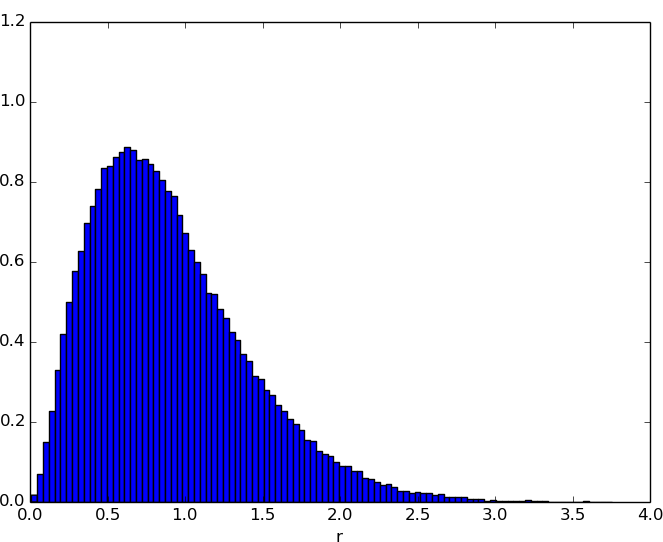
\includegraphics[width=0.32\linewidth]{content/Results/figures/ChargeDensityHelium_trimmed}
					\protect\caption{Radial densities of an helium atom simulated with different trial functions. From the left the plots represents pure hydrogenic wave functions, hydrogenic wave functions with an optimized alpha,  and hydrogenic wave functions with a Jastrow factor and optimized variational parameters.}
					\label{fig:HeliumoneBodyDensity}
					% ($\alpha = 2$, $E = -2.757$ and $\sigma^2_* = 0.0030$)
					% ($\alpha = 1.65$, $E = -2.843$ and $\sigma^2_* = 0.0027$)
					% ($\alpha = 1.843$, $\beta = 0.34$, $E = -2.887$, $\sigma^2_* = 0.0010$ )
					%  The simulations were run with \(10^6\) Monte Carlo cycles
			\end{figure}

			As expected, since the trialfunctions used here is based only on the \(\psi_{1S}\) orbitals, the radial distribution is similar to the \(\psi_{1S}\) hydrogen orbital in \ref{fig:orbitals_radial}.


		\subsubsection{Beryllium}
			There is a similar drop in the energy going from a purely hydrogenic wavefunction to a wavefunction where we have introduced a variational parameter, comparing values in Tabs. \ref{tab:helium_wavefunctions_tests} and \ref{tab:EnergyAlphaBetaReference}.
			The hydrogenic wavefunction for Beryllium consists of a Slater determinant constructed of the first two hydrogenic orbitals, plotted in Fig. \ref{fig:orbitals_radial}. The traces of the 1s orbital is there in the first maximum and is closer to the nucleus than in an hydrogen atom, which is expected since the distance is a function of the nucleus charge. The contribution from the second orbital 2s is visible as the second maximum in the distribution of Fig.~\ref{fig:oneBodyDensityBeryllium}. When the correlation factor is included the distribution is smeared out and the orbitals are not as sharply peaked.


			\begin{figure}
				\centering 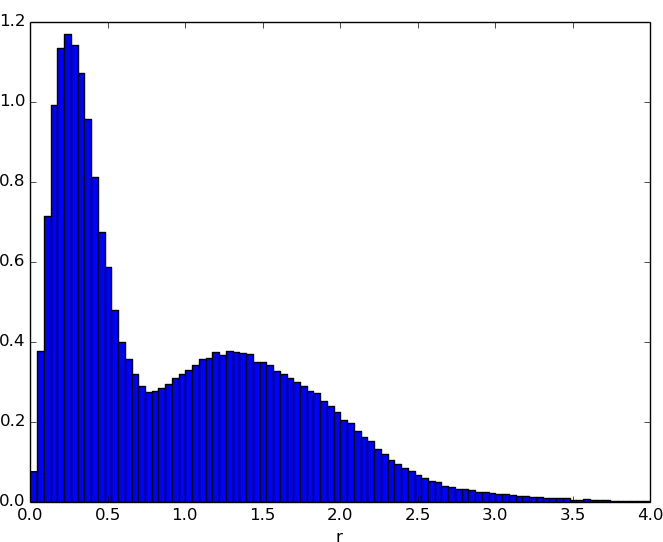
\includegraphics[width=0.49\linewidth]{content/Results/figures/ChargeDensityBerylliumSimple}
				\centering 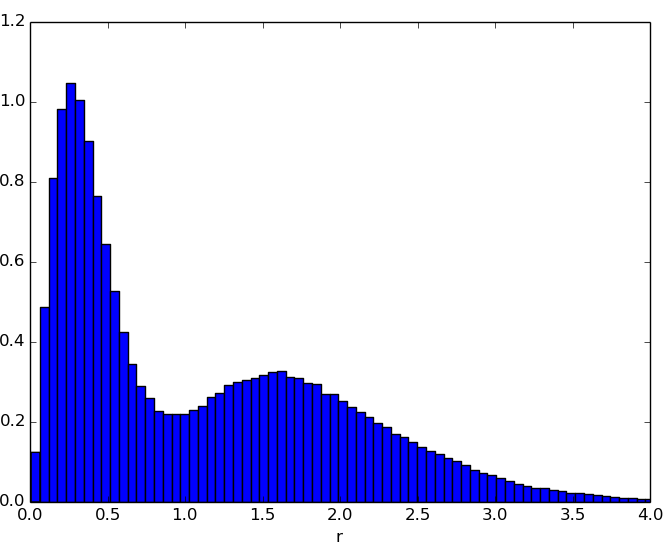
\includegraphics[width=0.49\linewidth]{content/Results/figures/ChargeDensityBeryllium}
				\protect\caption{The radial densities of a beryllium atom simulated with different trial functions. The left plot is with hydrogenic wave functions and the right plot is with hydrogenic wave functions using a Jastrow factor and optimized parameters.}
				\label{fig:oneBodyDensityBeryllium}
				% ($\alpha = 4$, $E = -13.710$, $\sigma^2_* = 0.0072$)
				% ($\alpha = 4$, $\beta = 0.31$,  $E = -14.385$, $\sigma^2_* = 0.0029$ )
			\end{figure}

			
		\subsubsection{Neon}
			As with helium and beryllium there is a drop
                        in the energy as we introduce a variational
                        parameter. The trial functions for neon
                        include all the three orbitals and the
                        distribution, presented in
                        Fig. \ref{fig:oneBodyDensityNeon} is
                        contracted closer to the nucleus than in the
                        other atoms. Here we can see the largest
                        effect due to the inclusion of the correlation
                        factor, both in the ground state energy and
                        the radial distribution. This is because the
                        electrons are closer together than in the
                        other atoms due to the higher charge of the
                        nucleus.
			\begin{figure}
				\centering 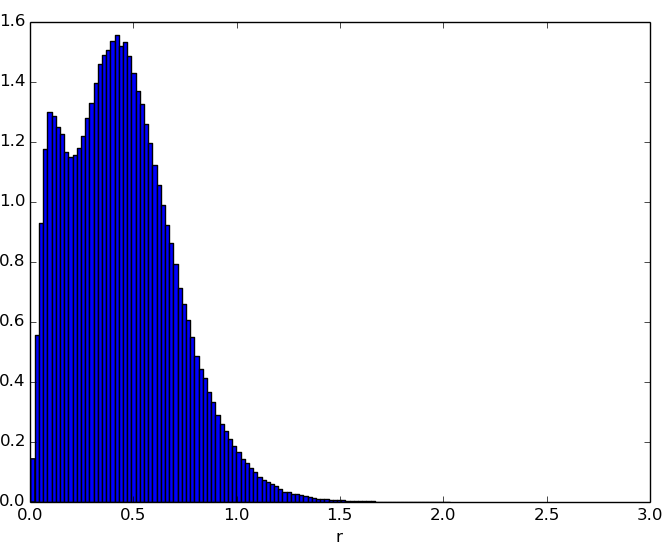
\includegraphics[width=0.49\linewidth]{content/Results/figures/ChargeDensityNeonSimple}
				\centering 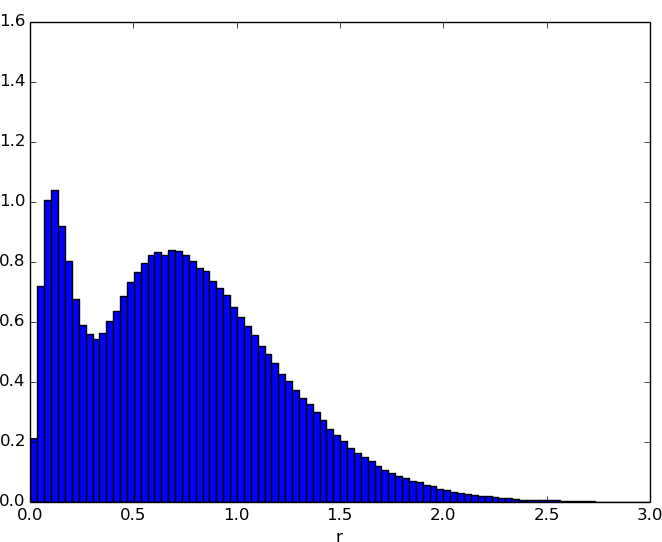
\includegraphics[width=0.49\linewidth]{content/Results/figures/ChargeDensityNeon}
				\protect\caption{Radial densities of an Neon atom simulated with different trial functions. The left plot is with hydrogenic wave functions and the right plot is with hydrogenic wave functions with a Jastrow factor and optimized parameters.}
				\label{fig:oneBodyDensityNeon}
				% ($\alpha = 10.22$, $E = -110.301$, $\sigma^2_* = 0.0477$)
				% ( $\alpha = 10.22$, $\beta = 0.0.091$,  $E = -127.888$, $\sigma^2_* = 0.0190$ )
				% The simulations were run with \(10^6\) Monte Carlo cycles
			\end{figure}

		\subsubsection{Hydrogen Molecule}
			Density plots for the hydrogen molecule
                        $H_{2}$ are presented in
                        Fig. \ref{fig:oneBodyDensityHydrogenTwo}. For
                        this molecule, which is comparable to a Helium
                        atom with the protons separated, the radial
                        distribution from the mass center appears
                        slightly more smeared out than in the Helium
                        atom because the protons are slightly apart.
                        In the one-body density plot, sliced about the
                        \(xz\) plane, the electron density around the
                        nuclei is higher. 

			\begin{figure}[H]
				\centering 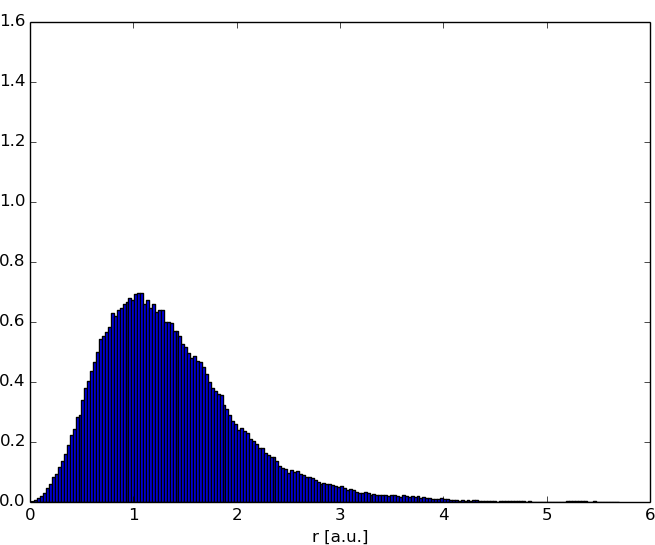
\includegraphics[width=0.32\linewidth]{content/Results/figures/ChargeDensityHydrogenTwo}
				\centering 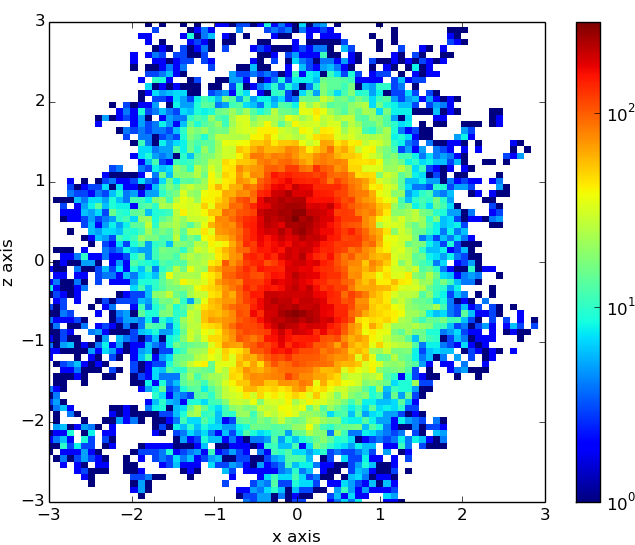
\includegraphics[width=0.32\linewidth]{content/Results/figures/OneBodyDensityHydrogenTwo}
				\centering 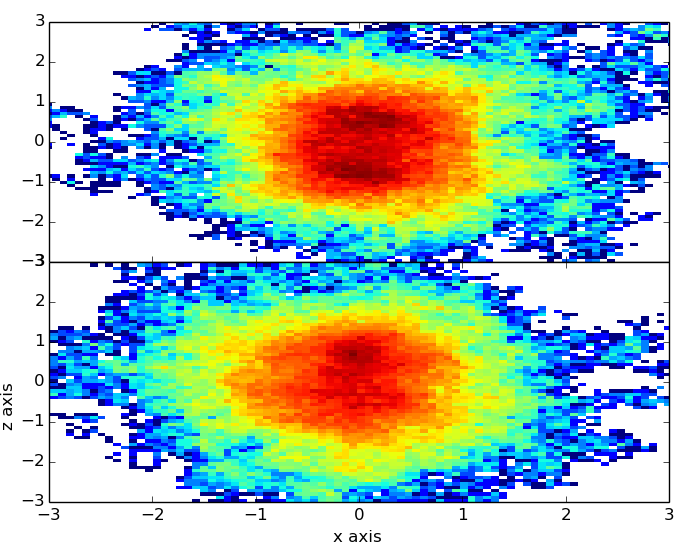
\includegraphics[width=0.32\linewidth]{content/Results/figures/OneBodyDensityElectronsHydrogenTwo}
				\protect\caption{On the left the the radial distribution of the hydrogen molecule is presented, where both nuclei are placed \(R = 1.40\) atomic units way from each other on the \(z\) axis. In the center a slice of the density in the \(xz\) plane with a width of \(1.0\) atomic units is shown. On the right one-body densities of each of the electrons are shown. Both the nuclei are visible on the one-body density plot as a denser concentration.}
				\label{fig:oneBodyDensityHydrogenTwo}
			\end{figure}



		\subsubsection{Beryllium Molecule}

			For the beryllium molecule, $Be_{2}$, shown in
                        Fig. \ref{fig:oneBodyDensityBerylliumTwo}, the
                        concentration of the one-body density around
                        the nuclei is sharper than in the hydrogen
                        molecule, which is likely caused by the higher
                        charge of the nuclei. In the beryllium atom we
                        also see that the electron density is higher
                        closer to the nucleus. The one-body density
                        plots here are not to be completely trusted
                        because there is a bug in the implementation
                        of the molecule which causes a too low binding
                        energy, but much of the expected physics still
                        seem to be captured by the VMC computation. By
                        following only one of the electrons in the
                        one-body densities presented in
                        Fig. \ref{fig:oneBodyDensityBerylliumTwo} we
                        can see that, compared to the Hydrogen
                        molecule, the nuclei in the molecule trap
                        the  electrons more efficiently.
			
			\begin{figure}[H]
				\centering 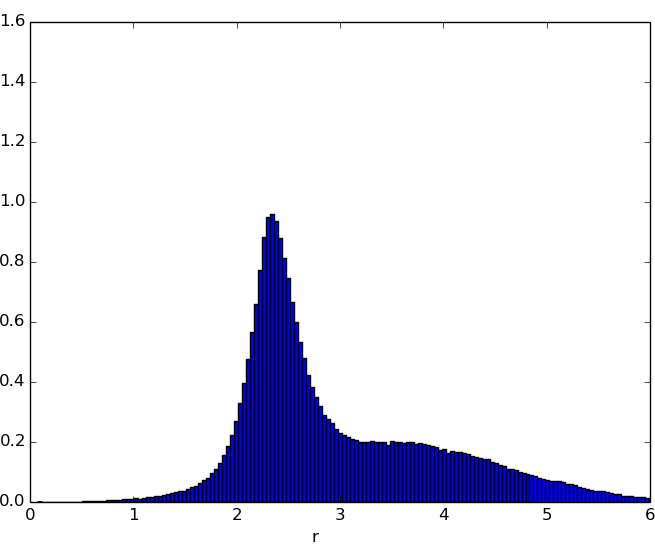
\includegraphics[width=0.32\linewidth]{content/Results/figures/ChargeDensityBerylliumTwo}
				\centering 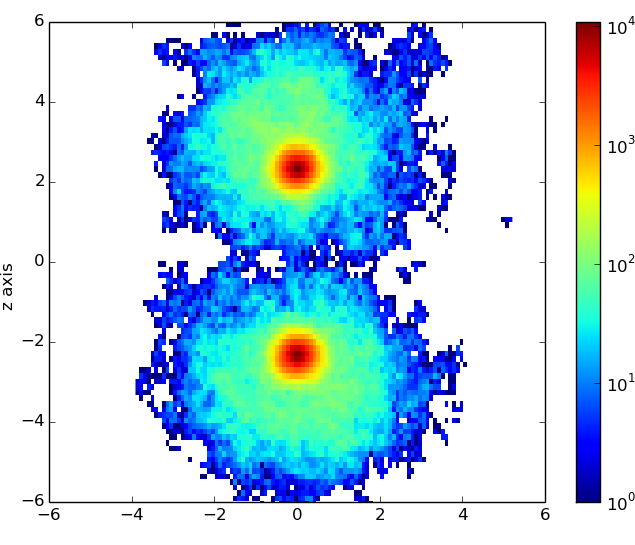
\includegraphics[width=0.32\linewidth]{content/Results/figures/OneBodyDensityBerylliumTwo}
				\centering 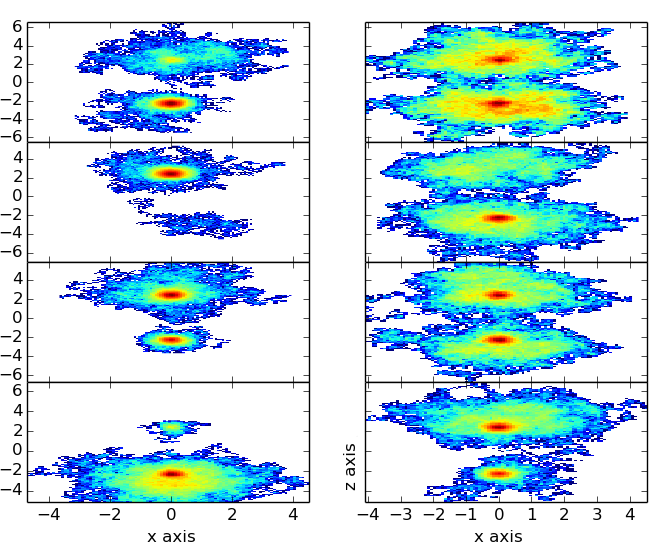
\includegraphics[width=0.32\linewidth]{content/Results/figures/OneBodyDensityElectronsBerylliumTwo}
				\protect\caption{On the left the radial distribution of the beryllium molecule is presented, where both nuclei where placed \(R = 4.63\) atomic units away from each other on the \(z\) axis. In the center the one-body density of a slice of density in the the \(xz\) plane with with of \(1.0\) atomic units is shown. On the right one-body densities of each of the electrons is shown. The concentration of the one-body density is very sharp around the two nuclei.}
				\label{fig:oneBodyDensityBerylliumTwo}
			\end{figure}

